\documentclass{ip-lab}

\usetikzlibrary{arrows.meta}

\lablevel{n1}
\labnumber{Laboratorio 4}
\labtitle{Pre parcial}

\makeheader

\begin{document}

\maketitle

\begin{sectionbox}{Preparación}
    Cree un nuevo archivo en Spyder denominado \texttt{parcialcito.py}. Las funciones de las Actividades 1 y 2 deben definirse en este módulo.
\end{sectionbox}

\begin{sectionbox}{Actividad 1: Optimización de billetes}
En Colombia, los billetes en circulación tienen las siguientes denominaciones: \$100.000, \$50.000, \$20.000, \$10.000, \$5.000, \$2.000 y \$1.000.

Defina una función que reciba como parámetro un monto entero en pesos colombianos (múltiplo de 1000) y retorne un \verb|str| indicando la cantidad mínima de billetes de cada denominación necesarios para completar dicho monto.
\end{sectionbox}

\begin{sectionbox}{Actividad 2: Esfera empacada en un cubo}
Considere una esfera de radio $r$ que se empaca en el cubo más pequeño que la puede contener.

\begin{center}
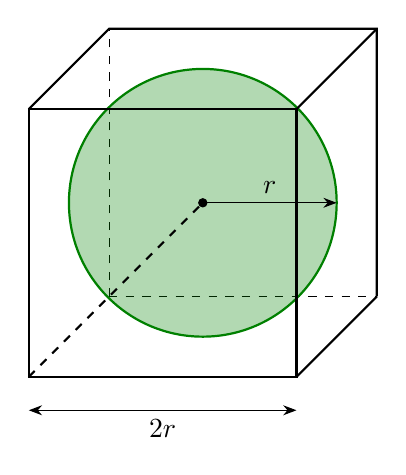
\begin{tikzpicture}[scale=0.85]
    % Back edges (dashed, drawn first)
    \draw[dashed] (0,0) -- (1.2,1.2);
    \draw[dashed] (1.2,1.2) -- (5.2,1.2);
    \draw[dashed] (1.2,1.2) -- (1.2,5.2);

    % Sphere (inside the cube)
    \fill[green!50!black, opacity=0.3] (2.6,2.6) circle (2);
    \draw[thick, green!50!black] (2.6,2.6) circle (2);

    % Front face
    \draw[thick] (0,0) -- (4,0) -- (4,4) -- (0,4) -- cycle;

    % Top and right connecting edges
    \draw[thick] (4,0) -- (5.2,1.2);
    \draw[thick] (5.2,1.2) -- (5.2,5.2) -- (1.2,5.2) -- (0,4);
    \draw[thick] (4,4) -- (5.2,5.2);

    % Diagonal from front-bottom-left corner to center
    \draw[dashed, thick] (0,0) -- (2.6,2.6);

    % Center point
    \fill (2.6,2.6) circle (2pt);

    % Radius arrow
    \draw[-{Stealth}] (2.6,2.6) -- (4.6,2.6) node[midway, above] {$r$};

    % Side label
    \draw[{Stealth}-{Stealth}] (0,-0.5) -- (4,-0.5) node[midway, below] {$2r$};
\end{tikzpicture}
\end{center}

Defina una función que reciba como parámetro el radio $r$ de la esfera y retorne la distancia más corta desde una esquina del cubo hasta la superficie de la esfera.

Aproxime la respuesta a dos decimales.

\textbf{Consejo:} El segmento más corto desde la esquina del cubo hasta la esfera está contenido en la diagonal espacial del cubo
\end{sectionbox}

\pagebreak

\begin{sectionbox}{Actividad 3: Capa de presentación}
Para cada función de la capa de lógica, escriba el módulo de la capa de presentación. Es decir:
\begin{enumerate}
    \item Cree un módulo que importe el módulo de lógica, solicite al usuario un monto en pesos y muestre el desglose de billetes correspondiente.
    \item Cree otro módulo similar al anterior que solicite al usuario el radio de una esfera y muestre la distancia desde una esquina del cubo hasta el punto más cercano de la esfera.
\end{enumerate}
\end{sectionbox}

\begin{sectionbox}{Actividad 4: Pruebas}
Ejecute cada consola para probar que el programa funciona. Puede usar los siguientes valores de prueba:
\begin{itemize}
  \item Para el desglose de billetes, un monto de \verb|378_000| pesos debería arrojar: 3 de \$100.000, 1 de \$50.000, 1 de \$20.000, 0 de \$10.000, 1 de \$5.000, 1 de \$2.000 y 1 de \$1.000.
  \item Para la esfera empacada, un radio de \verb|5| debería dar una distancia de aproximadamente \verb|3.66|.
\end{itemize}
\end{sectionbox}

\begin{sectionbox}{Entrega}
  Cree un archivo comprimido .zip que contenga exactamente el módulo de la capa de lógica y los módulos de la capa de presentación. Entregue el archivo comprimido a través de Bloque Neón en el laboratorio del Nivel 1 designado como ``L4: Pre parcial''.
\end{sectionbox}

\end{document}
